\documentclass{standalone}
\usepackage[utf8]{inputenc}
\usepackage[a-3b,mathxmp]{pdfx}
\usepackage{pgfplots}
\usepackage{amsmath}

\pgfplotsset{compat=newest}
\usetikzlibrary{patterns.meta}
\usepgfplotslibrary{fillbetween}

\begin{document}
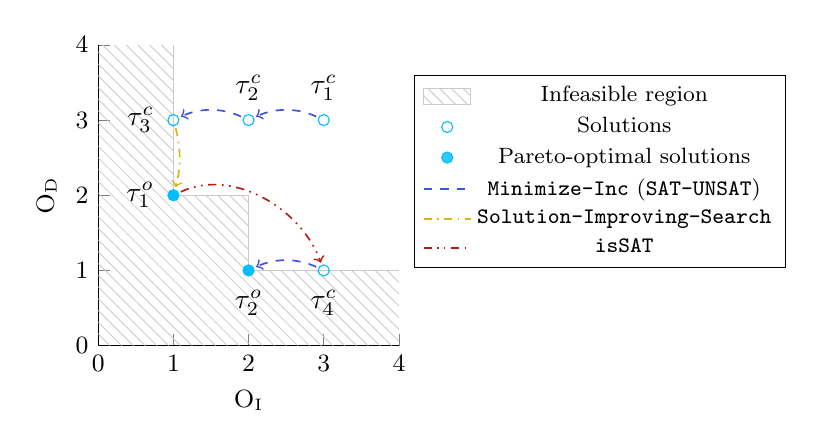
\begin{tikzpicture}

% xfgs_normal6 colour palette
\definecolor{color0}{RGB}{64,83,211}
\definecolor{color1}{RGB}{221,179,16}
\definecolor{color2}{RGB}{181,29,20}
\definecolor{color3}{RGB}{0,190,255}
\definecolor{color4}{RGB}{251,73,176}
\definecolor{color5}{RGB}{0,178,93}
\definecolor{color6}{RGB}{202,202,202}

% xgfs_normal12 colour palette
%\definecolor{color0}{RGB}{235,172,35}
%\definecolor{color1}{RGB}{184,0,88}
%\definecolor{color2}{RGB}{0,140,249}
%\definecolor{color3}{RGB}{0,110,0}
%\definecolor{color4}{RGB}{0,187,173}
%\definecolor{color5}{RGB}{209,99,230}
%\definecolor{color6}{RGB}{178,69,2}
%\definecolor{color7}{RGB}{255,146,135}
%\definecolor{color8}{RGB}{89,84,214}
%\definecolor{color9}{RGB}{0,198,248}
%\definecolor{color10}{RGB}{135,133,0}
%\definecolor{color11}{RGB}{0,167,108}
%\definecolor{color12}{RGB}{189,189,189}

% xfgs_fancy6 colour palette
%\definecolor{color0}{RGB}{86,100,26}
%\definecolor{color1}{RGB}{192,175,251}
%\definecolor{color2}{RGB}{230,161,118}
%\definecolor{color3}{RGB}{0,103,138}
%\definecolor{color4}{RGB}{152,68,100}
%\definecolor{color5}{RGB}{94,204,171}
%\definecolor{color6}{RGB}{205,205,205}

% paultol_muted colour palette
%\definecolor{color0}{RGB}{204,102,119}
%\definecolor{color1}{RGB}{51,34,136}
%\definecolor{color2}{RGB}{221,204,119}
%\definecolor{color3}{RGB}{17,119,51}
%\definecolor{color4}{RGB}{136,204,238}
%\definecolor{color5}{RGB}{136,34,85}
%\definecolor{color6}{RGB}{68,170,153}
%\definecolor{color7}{RGB}{153,153,51}
%\definecolor{color8}{RGB}{170,68,153}

% paultol_bright colour palette
%\definecolor{color0}{RGB}{68,119,170}
%\definecolor{color1}{RGB}{102,204,238}
%\definecolor{color2}{RGB}{34,136,51}
%\definecolor{color3}{RGB}{204,187,68}
%\definecolor{color4}{RGB}{238,102,119}
%\definecolor{color5}{RGB}{170,51,119}
%\definecolor{color6}{RGB}{187,187,187}

\newcommand{\formula}{F}
\newcommand{\Obj}{\textsc{O}}
\newcommand{\inc}{\text{I}}
\newcommand{\dec}{\text{D}}
\newcommand{\var}{\textsc{var}}
\newcommand{\lit}{\textsc{lit}}
\newcommand{\Min}{\texttt{Minimize-\allowbreak{}Inc}}
\newcommand{\Simpr}{\texttt{Solution-\allowbreak{}Improving-\allowbreak{}Search}}
\newcommand{\E}{\texttt{EnumSols}}
\newcommand{\Ex}{\texttt{ExistsSol}}
\newcommand{\T}{\mathtt{T}}
\newcommand{\assumps}{\mathcal{A}}
\newcommand{\satsolver}{\texttt{isSAT}}
\newcommand{\res}{\text{res}}
\newcommand{\algname}{\textsc{BiOptSat}}
\newcommand{\tot}{\textsc{Tot}}
\newcommand{\ov}[2]{\langle #1 < #2 \rangle}
\newcommand{\ove}[2]{\langle #1 \leq #2 \rangle}
\newcommand{\satunsat}{\texttt{SAT-\allowbreak{}UNSAT}}
\newcommand{\unsatsat}{\texttt{UNSAT-\allowbreak{}SAT}}
\newcommand{\msu}{\texttt{MSU3}}
\newcommand{\I}{\mathcal{I}}
\newcommand{\Act}{\texttt{Act}}
\newcommand{\oll}{\texttt{OLL}}
\newcommand{\msh}{\texttt{MSHybrid}}
\newcommand{\hs}{\texttt{hs}}
\newcommand{\nsamp}{n}
\newcommand{\nfeat}{m}
\newcommand{\nclauses}{k}
\newcommand{\selector}{s}
\newcommand{\noise}{\eta}
\newcommand{\equals}{e}
\newcommand{\nelems}{n}
\newcommand{\nsets}{m}
\newcommand{\setcard}{s}
\newcommand{\elemprob}{p}
\newcommand{\sets}{\mathcal{S}}
\newcommand{\element}{e}
\newcommand{\cover}{\mathcal{C}}
\newcommand{\cost}{c}
\newcommand{\cores}{\mathcal{K}}
\newcommand{\core}{\kappa}
\newcommand{\sol}{\tau}
\newcommand{\scep}{SetCovering-EP}
\newcommand{\scsc}{SetCovering-SC}
\newcommand{\clause}{C}
\newcommand{\softs}{\textsc{S}}
\newcommand{\generalobj}{f}
\newcommand{\nobj}{p}
\newcommand{\feasible}{\mathcal{X}}
\newcommand{\decvar}{x}
\newcommand{\soloone}{\{i_2,\allowbreak d_1,\allowbreak d_3,\allowbreak d_4,\allowbreak \lnot i_1,\allowbreak \lnot i_3,\allowbreak \lnot i_4,\allowbreak \lnot d_2\}}
\newcommand{\solotwo}{\{i_1,\allowbreak i_2,\allowbreak d_1,\allowbreak d_2,\allowbreak \lnot i_3,\allowbreak \lnot i_4,\allowbreak \lnot d_3,\allowbreak \lnot d_4\}}
\newcommand{\solothree}{\{i_2,\allowbreak d_1,\allowbreak d_3,\allowbreak d_4,\allowbreak \lnot i_1,\allowbreak \lnot i_3,\allowbreak \lnot i_4,\allowbreak \lnot d_2\}}
\newcommand{\solcone}{\{i_1,\allowbreak i_2,\allowbreak i_3,\allowbreak i_4,\allowbreak d_1,\allowbreak d_2,\allowbreak d_3,\allowbreak d_4\}}
\newcommand{\solctwo}{\{i_1,\allowbreak i_2,\allowbreak d_1,\allowbreak d_2,\allowbreak d_3,\allowbreak d_4,\allowbreak \lnot i_3,\allowbreak \lnot i_4\}}
\newcommand{\solcthree}{\{i_2,\allowbreak d_1,\allowbreak d_2,\allowbreak d_3,\allowbreak d_4,\allowbreak \lnot i_1,\allowbreak \lnot i_3,\allowbreak \lnot i_4\}}
\newcommand{\solcfour}{\{i_1,\allowbreak i_2,\allowbreak i_3,\allowbreak d_1,\allowbreak d_2,\allowbreak \lnot i_4,\allowbreak \lnot d_3,\allowbreak \lnot d_4\}}
\newcommand{\solmcstrap}{\{i_1,\allowbreak i_3,\allowbreak i_4,\allowbreak d_1,\allowbreak d_3,\allowbreak d_4,\allowbreak \lnot i_2,\allowbreak \lnot d_2\}}
\newcommand{\TODO}[1]{\textcolor{red}{#1}}
\newcommand{\thr}{\texttt{thr}}
\newcommand{\NP}{$\mathcal{NP}$}

\begin{axis}[
  width=5.4cm,
  height=5.4cm,
  label style={font=\small},
  tick label style={font=\small},
  legend style={
    anchor=north west,
    at={(1.05,0.9)},
    font=\footnotesize,
    fill opacity=0.8,
    draw opacity=1,
    text opacity=1
  },
  tick pos=left,
  xlabel={$\textsc{O}_\text{I}$},
  ylabel={$\textsc{O}_\text{D}$},
  xmin=0,
  xmax=4,
  ymin=0,
  ymax=4,
  axis x line*=bottom,
  axis y line*=left,
  xtick={0,1,2,3,4},
  ytick={0,1,2,3,4},
]

\addplot [color6,name path=border,forget plot] coordinates {(1,4) (1,2) (2,2) (2,1) (4,1)};
\path [name path=axis] (1,4) -- (0,4) -- (0,0) -- (4,0) -- (4,1);
\addplot [color6,pattern={Lines[angle=-45, line width=.3pt]}, pattern color=color6] fill between [of=border and axis];
\addlegendentry{Infeasible region}

\draw [semithick,dashed, color0, ->, shorten >=3pt, shorten <=3pt] (3,3) to[out=155, in=25] (2,3);
\draw [semithick,dashed, color0, ->, shorten >=3pt, shorten <=3pt] (2,3) to[out=155, in=25] (1,3);
\draw [semithick,dashdotted, color1, ->, shorten >=3pt, shorten <=3pt] (1,3) to[out=-75, in=75] (1,2);
\draw [semithick,dashdotdotted, color2, ->, shorten >=3pt, shorten <=3pt] (1,2) to[out=25, in=110] (3,1);
\draw [semithick,dashed, color0, ->, shorten >=3pt, shorten <=3pt] (3,1) to[out=155, in=25] (2,1);

\addplot [only marks,color3, mark=o] coordinates {(3,3) (2,3) (1,3) (3,1)};
\addlegendentry{Solutions}

\addplot [only marks,color3, mark=*] coordinates {(1,2) (2,1)};
\addlegendentry{Pareto-optimal solutions}

\addlegendimage{color0,dashed,semithick}
\addlegendentry{\Min{} (\satunsat{})}

\addlegendimage{color1,dashdotted,semithick}
\addlegendentry{\Simpr{}}

\addlegendimage{color2,dashdotdotted,semithick}
\addlegendentry{\satsolver{}}

\node [label=$\tau^c_1$] at (3,3) {};
\node [label=$\tau^c_2$] at (2,3) {};
\node [label=left:$\tau^c_3$] at (1,3) {};
\node [label=left:$\tau^o_1$] at (1,2) {};
\node [label=below:$\tau^c_4$] at (3,1) {};
\node [label=below:$\tau^o_2$] at (2,1) {};

\end{axis}
\end{tikzpicture}
\end{document}